I denne opgave skal du arbejde med brætspillet Dam og objektorienteret programmering og design i F\#.

Spillet er som følger:
\begin{quote}
  Dam spilles af 2 spillere på et ternet bræt med lyse og mørke felter. Ved start får hver spiller 12 brikker i hhv.\ lys og mørk farve, og brikkerne anbringes i de 3 første rækker på de mørke felter over for hinanden, som vist nedenfor.
  \begin{center}
    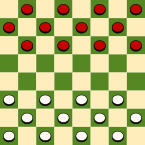
\includegraphics[width=0.3\textwidth]{145px-Draughts}
  \end{center}
  Der spilles kun på de mørke felter, og brikken flyttes skråt fremad et felt ad gangen.

  Modstanderens brikker slås, hvis disse støder op til ens egne med et tomt felt skråt bagved. Flere brikker kan slås i samme træk, bare der hele tiden er et tomt felt bag den brik, som erobres. Man kan skifte retning for hver brik man har slået, så længe man bevæger sig fremad.

  Lykkes det at komme frem til modstanderens bageste række, opnår man en dam. Denne brik markeres ved at placere en af ens slagne brikker ovenpå. En dam kan flyttes på skrå lige så mange felter frem eller tilbage, som der er tomme felter, og slå modstanderens brikker som tidligere.

  Spilleren, der har slået alle modstanderens brikker, eller har lukket dem inde, så de ikke kan flyttes, har vundet
\end{quote}

I denne opgave skal du lave en skitse til at program, hvor 2 spillere kan spille Dam med hinanden på en computer. Dertil skal du lave følgende opgaver:
\begin{itemize}
\item Identificer nyttige klasser og metoder vha.\ navne- og udsagnsordsmetoden
\item Tegn et UML diagram til et udkast til et design for spillet.
\item Skriv et mockup program i F\#, som implementerer dit design med alle de klasser og metoder, som dit design indeholder og med korte kommentarer om de væsentlige opgaver, som hver klasse og metode har i programmet.  
\end{itemize}
